\documentclass{article}
\usepackage[utf8]{inputenc}
\usepackage{newspaper}
\date{\today}
\currentvolume{1}
\currentissue{1}

\usepackage{graphicx} % Required for including images
\usepackage{lipsum} % Package to generate dummy text throughout this template
\usepackage[english]{babel} % Language hyphenation and typographical rules
\usepackage{multicol} % Used for the two-column layout of the document

\SetPaperName{Global Health}
\SetHeaderName{GH News}
\SetPaperSlogan{``Your source for worldwide health insights''}
\SetPaperPrice{Free}

\begin{document}
\maketitle

\begin{multicols}{2}
[\textbf{\huge Beneficial Bio: Enabling Local Diagnostics}]
\byline{\textbf{An In-Depth Analysis}}{Fran Quero }
In 2021, during the latter half of the Covid-19 pandemic, Médecins Sans Frontières published in their article ``Local Diagnostics to Meet Local Health Needs" 
a significant analysis of how the centralization of diagnostic method production on high-income countries (HICs) was creating extensive dependency chains,
 hindering distributed industrial development, and favoring an unsustainable economy. As the pandemic demonstrated, a global demand for diagnostics faces serious 
 issues when addressed solely by the production capacity of HICs.

The Médecins Sans Frontières briefing included a list of local diagnostic test producers and a global distribution map. I have recently visited some of these companies,
 which typically focused on bulk purchasing and repackaging foreign products, to find that there's a growing trend to adopt on-site production processes. An example is 
 the production of lateral flow chromatography rapid tests, whose the design, assembly, quality control, and certification
  are increasingly being handled locally (although they still rely on reagents from HICs).

Médecins Sans Frontières is clear on the necessary changes; there must be a global effort in developing open source technologies that allow rapid and flexible adoption, 
production, and certification by actors in Low and Middle Income Countries (LMICs).

In 2019, Dr. Jenny Molloy and Cesar Gomez, supported by the Shuttleworth Foundation, founded Beneficial Bio Ltd., a non-profit dedicated to developing Open Source methods and materials for local production
of en-
\begin{center}
  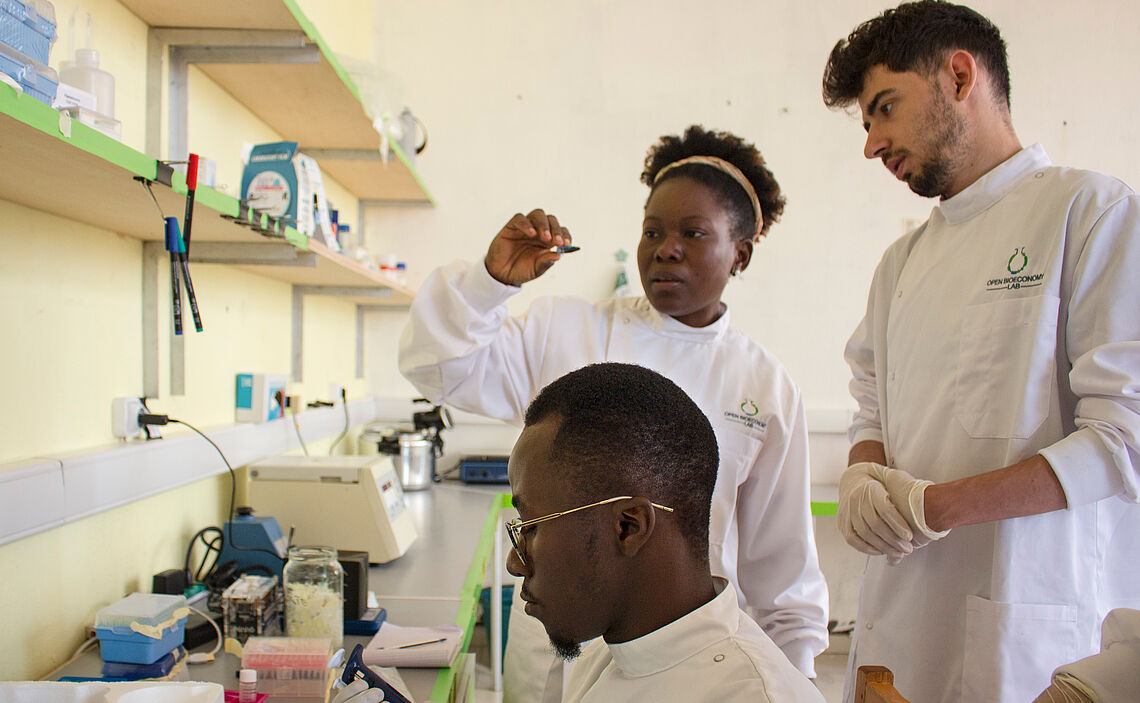
\includegraphics[width=\linewidth]{lab.jpg}
\end{center}
\columnbreak

zymes and diagnostic reagents, with a particular focus on cost-effective and easily adaptable methods for producing 
off-patent enzymes in low-infrastructure settings. 

\begin{center}
  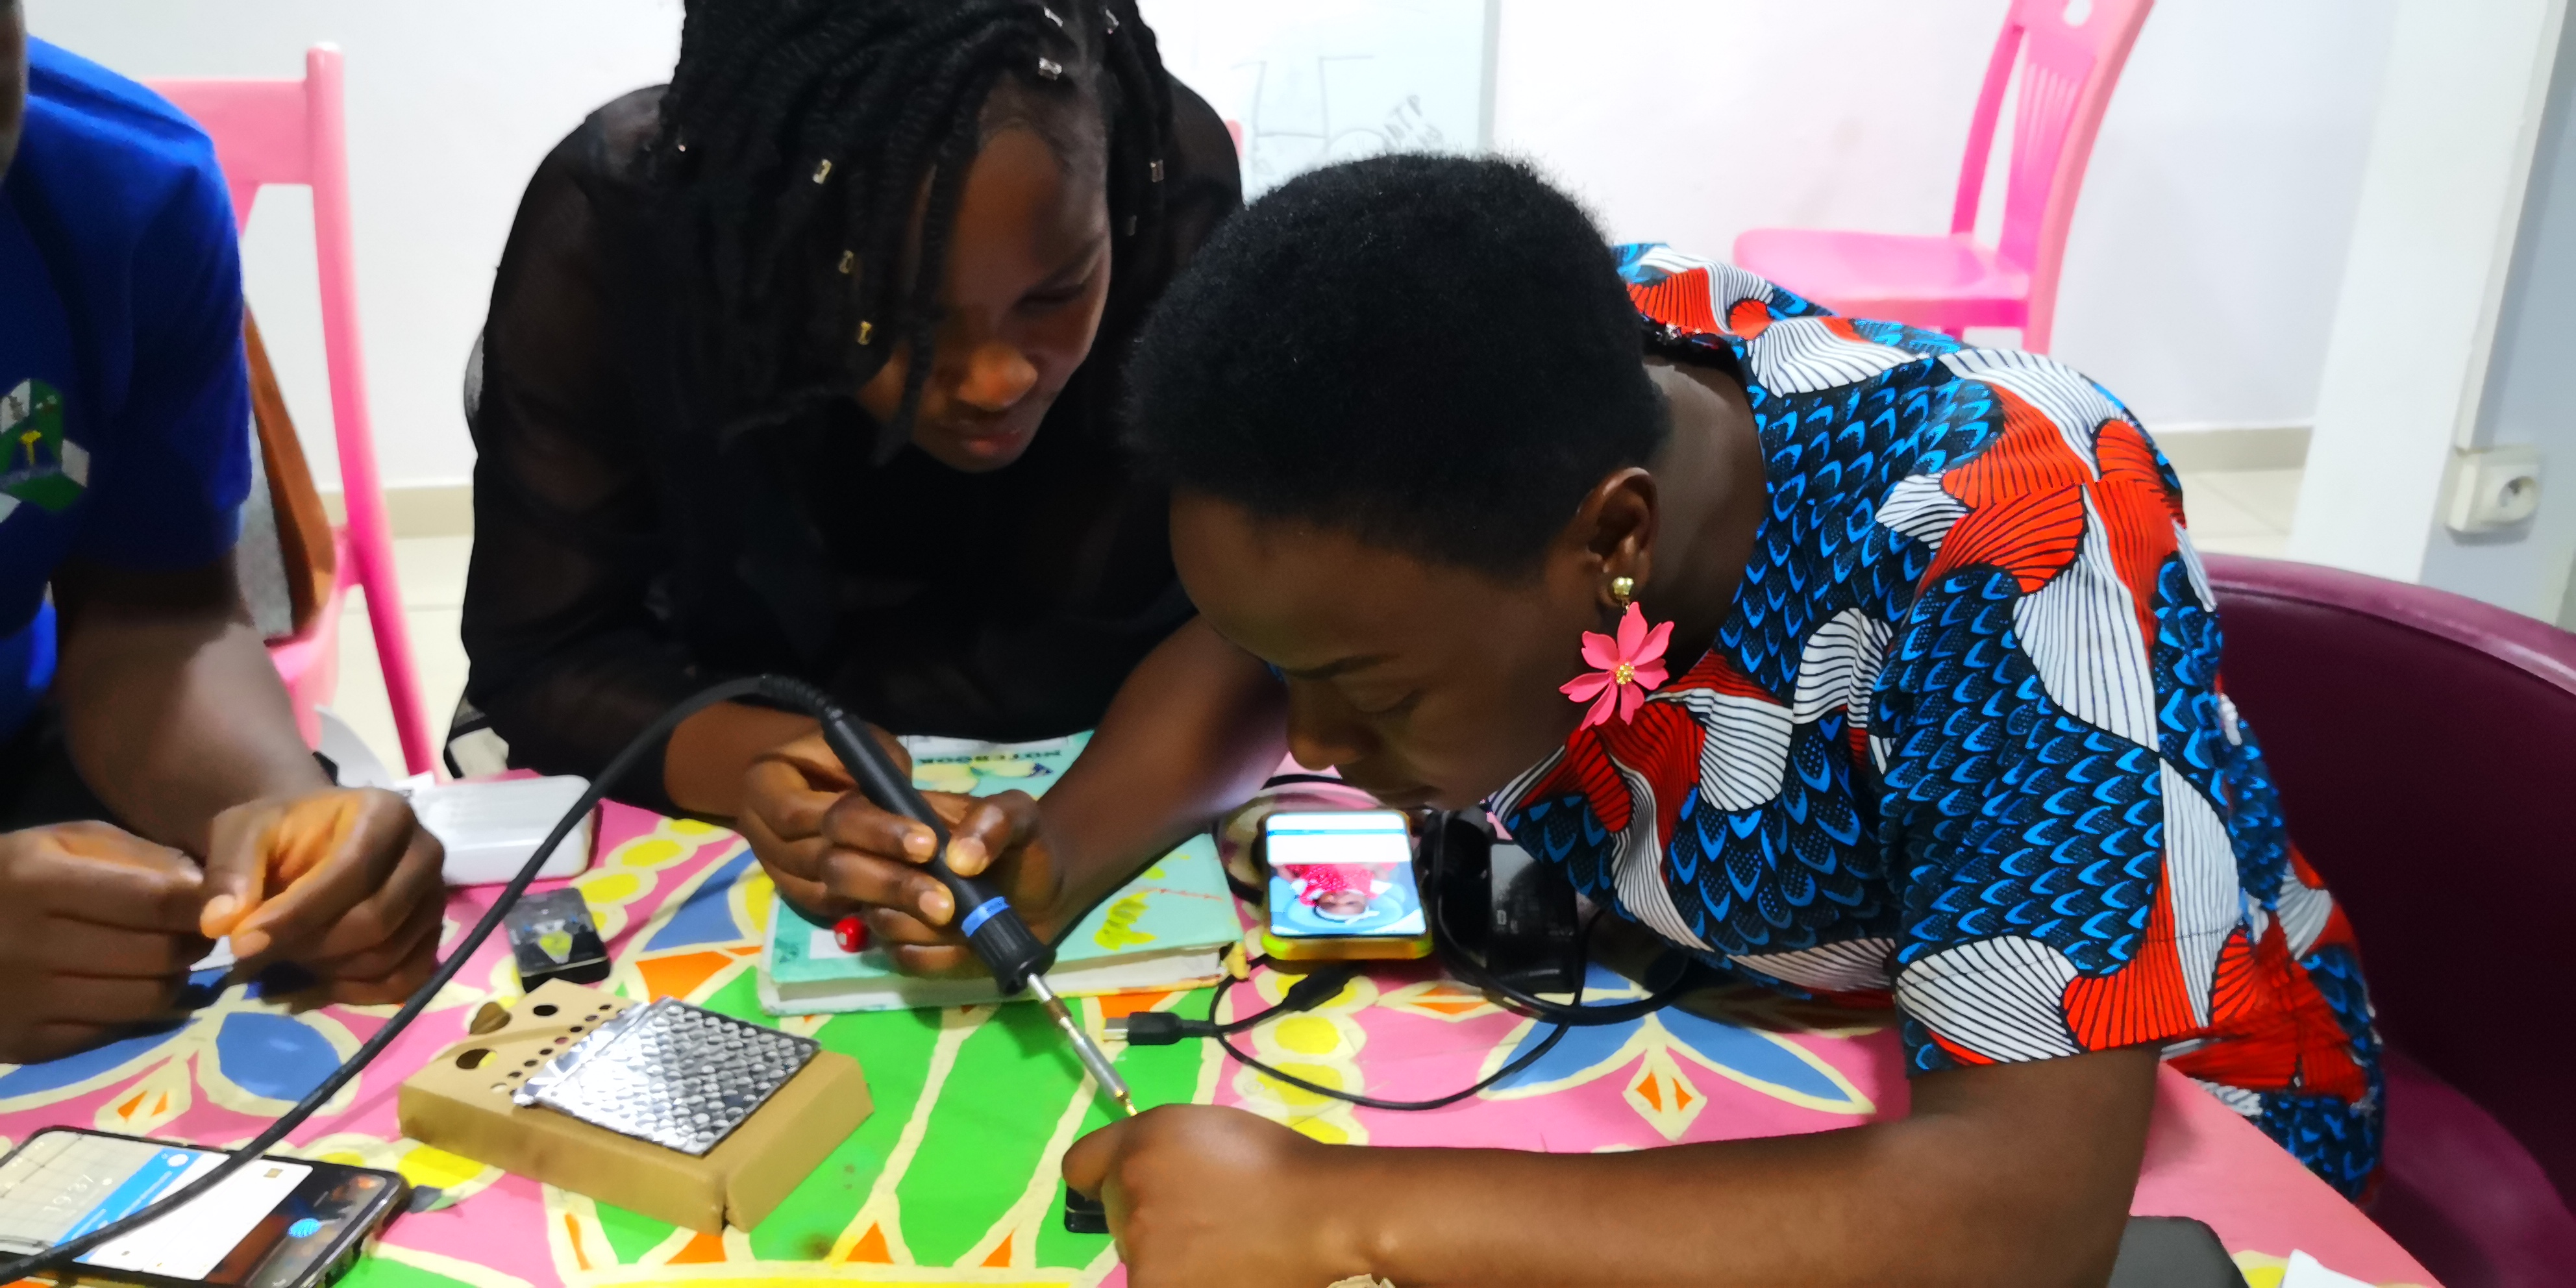
\includegraphics[width=\linewidth]{minette.jpg}
\end{center}

To promote the widespread adoption of these protocols and ease the implementation of these techniques by local partners, 
Beneficial Bio places a strong emphasis on developing training programs in molecular biology techniques and establishing collaborative networks where different nodes or 
members can freely share advancements and new developments.

Despite being quite new, Beneficial Bio has already shown very promising results. One of its first pilot collaborations with Mboalab, created by Thomas Mboa in Yaoundé, 
Cameroon, has grown in recent years as a robust alternative in the enzyme and reagent market in the region. When I first visited Mboalab in 2018, it was a community 
laboratory set up in a small neighborhood on the outskirts of Cameroon. At that time, the lab was just starting, and was essentially two small spaces inside an old 
family house. A small maker lab with a 3D printer and basic tools, and a molecular biology lab with open source hardware and repurposed old machines.

Recently, I had the incredible opportunity to return to Mboalab following the Africa Open Source Hardware Conference. The change over the last 5 years is striking; 
the laboratory has expanded to a much larger room in the back where the team has established an "Enzyme Production Lab" for nucleic acid detection methods (PCR, LAMP, etc.), 
while the old lab remains as a Community Biolab where people from the region can come to learn molecular biology or use it to prototype their projects. Additionally, two new 
floors are being constructed for resident researchers, and a substantial "African Literature" library has been added. Mboalab is evolving towards a sustainable model, 
supplying enzymes to regional research centers and labs, not only with more competitive pricing but also with significantly shorter delivery times and enhanced customer service.

Mboalab was the first collaboration of Beneficial Bio, but now that it's self-sustaining, the focus has shifted to new partners in Latin America, Southeast Asia, and Sub-Saharan 
Africa. Beneficial Bio's goal is clear: to help bridge the gap in adapting, translating, and producing new diagnostic technologies in regions far from the world's major production 
zones. Gradually, Beneficial Bio is forging local partnerships with stakeholders eager to embrace these technologies. With the backing of already validated cases like Mboalab, they 
are progressively scaling their support and incubation model, aiming to make a significant impact in global health.

\end{multicols}

\end{document}

